% Gemini theme
% https://github.com/anishathalye/gemini

\documentclass[final,notheorems]{beamer}

% ====================
% Packages
% ====================

\usepackage[T1]{fontenc}
\usepackage{lmodern}
\usepackage[size=custom,width=120,height=72,scale=1.0]{beamerposter}
\usetheme{gemini}
\usecolortheme{ppposter}
\usepackage{graphicx}
\usepackage{booktabs}
\usepackage{tikz}
\usepackage{pgfplots}
\usepackage{amsmath}
\usepackage[backend=biber,maxcitenames=4,maxbibnames=99,giveninits=false]{biblatex}
\usepackage{xcolor}
\usepackage{siunitx}
\setbeamertemplate{theorems}[numbered] % to number

\addbibresource{poster.bib}

% ====================
% Lengths
% ====================

% If you have N columns, choose \sepwidth and \colwidth such that
% (N+1)*\sepwidth + N*\colwidth = \paperwidth
\newlength{\sepwidth}
\newlength{\colwidth}
\setlength{\sepwidth}{0.025\paperwidth}
\setlength{\colwidth}{0.3\paperwidth}

\newcommand{\separatorcolumn}{\begin{column}{\sepwidth}\end{column}}

% ====================
% Commands
% ====================
\providecommand{\abs}[1]{\lvert#1\rvert}
\providecommand{\norm}[1]{\lVert#1\rVert}
\def\bfx{\mathbf x}
\def\bfv{\mathbf v}
\def\X{\mathcal X}
\def\R{\mathbb R}

\newtheorem{imp}{Implication}

\definecolor{highlightbg}{HTML}{fcd588}


% ====================
% Title
% ====================

\title{Human Perception of Adversarial Images}

\author{Ayon Sen \inst{1} \and Xiaojin Zhu \inst{1} \and Liam Marshall \inst{1} \and Robert Nowak \inst{1}}

\institute[shortinst]{\inst{1} University of Wisconsin-Madison}

\addtobeamertemplate{headline}{}
{
    \begin{tikzpicture}[remember picture,overlay]
    \node [anchor=north east, inner sep=2cm] at ([xshift=1.4cm,yshift=1.4cm]current page.north east)     {
\includegraphics[height=6.5cm]{fig/black-flush-UWlogo-print.eps}};
    \end{tikzpicture}
}
% ====================
% Body
% ====================

\begin{document}

\begin{frame}[t]
\begin{columns}[t]
\separatorcolumn

\begin{column}{.6\colwidth}
  \begin{block}{Overview}
    Adversarial attacks attempt to confound machine learning systems. By changing the input to a classifier slightly -- for instance, tweaking image pixels -- the output classification can be manipulated.

    Throughout the literature on attacking image classifiers, the \emph{visibility} of attacks to a human observer (who might become \emph{suspicious}, which we wish to avoid) is typically gauged by a $p$-norm of the difference between the original and modified image.

    However, this has not been previously justified as an accurate model of human behavior.
    Via behavioral experiments, we show\cite{sen2019perception} that \textbf{human perception of image modifications is not well-described by \emph{any} $p$-norm, nor several alternative measures}.
    This has significant impact on adversarial ML research; the robustness of attacks to human inspection relies on an accurate understanding of \emph{what humans will and will not see as "tampering"}.

    \begin{figure}
      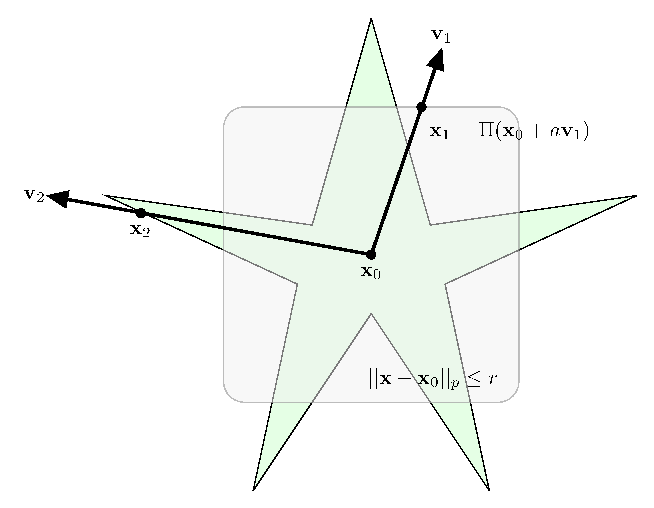
\includegraphics[width=.8\linewidth]{fig/intro_image-figure0.eps}
      \caption{Current research assumes a $p$-norm decision boundary (grey) on whether an image has been tampered with. The true human decision boundary (green) may be very different.}
      \label{fig:decision_boundary}
    \end{figure}
  \end{block}

  \begin{alertblock}{The current assumption}
    An image $\bfx_0$ sits in a pixel feature space $\X = \{0,\ldots,255\}^d$, where $d$ = $\text{\# pixels} \times \text{\# color channels}$ (assuming a color depth of 255).

    An adversarial attack perturbs this $\bfx_0$ into $\bfx$. Currently, the \textbf{general assumption} in adversarial image attacks is that:

    \hspace*{.1\linewidth}\colorbox{highlightbg}{\begin{minipage}{.8\linewidth}
      There exists some global $p>0$ and some $r$ (dependent on $\bfx_0$) where the observer perceives all $\bfx$ as visually identical to $\bfx_0$ as long as $\norm{\bfx_0-\bfx}_p < r(x_0)$ is satisfied.
    \end{minipage}}

    We refute this assumption via \emph{testable implications}.
  \end{alertblock}
\end{column}

\separatorcolumn

\begin{column}{\colwidth}
    \begin{block}{A weak implication}
    We define $J(\bfx_0) = \{\bfx \subset \X : \norm{\bfx_0-\bfx}_p = r(\bfx_0)\}$ as the set of all images just-noticeably-different from the base image $\bfx_0$.

    \hspace*{.1\linewidth}\colorbox{highlightbg}{\begin{minipage}{.8\linewidth}
      Supposing $p^*$ is the true value of $p$, for any pair of $\bfx_1$, $\bfx_2$ $\in J(\bfx_0)$, $\norm{\bfx_1-\bfx_0}_{p^*} = \norm{\bfx_2-\bfx_0}_{p^*}$.
    \end{minipage}}

    We can ask humans when they 'just notice' changes to an image and compare these judgments across $\bfx_1$, $\bfx_2$ pairs, but this implication is still \emph{weak} as a statistical test; it \emph{requires knowledge of the true $p^*$}.
  \end{block}

  \begin{block}{A stronger implication}
    Throughout our experiments, we generate images as in Figure~\ref{fig:decision_boundary};
    each image $\bfx = \Pi(\bfx_0+a\bfv)$ is defined by a ray or \textbf{perturbation direction} $\bfv \in \R^d$ and a \textbf{perturbation scale} $a>0$.
    $\Pi$ is the projection onto $\X$ (clipping and rounding).

    We construct \textbf{$\pm 1$-perturbation directions} as $\bfv\in\R^d$ where
    (i) $\bfv$ has $s>0$ nonzero elements, and
    (ii) nonzero elements $v_i = 1$ if $v_0,i < 128$ and $=-1$ otherwise.

    It is then possible to extract a new implication:

    \hspace*{.1\linewidth}\colorbox{highlightbg}{\begin{minipage}{.8\linewidth}
      If two perturbation directions $\bfv_1$, $\bfv_2$ have the same sparsity $s$, the perturbation scales $a_1$, $a_2$ at which humans notice changes must be equal.
    \end{minipage}}

    This is a particularly nice implication to test, because it only depends on having pairs of perturbation directions and judgements for them.
    If the equality hypothesis fails, \emph{no} $p$-norm is appropriate for modeling human perception of just-noticable-difference.
  \end{block}

  \begin{block}{Experimental design}
    We generate perturbation rays $\bfv$ on top of three natural images (cat, panda, macaw) from Imagenet.
    Eight rays are specially-crafted $\pm1$-perturbation directions varying in size, number of color channels affected, and shape of perturbed pixels.
    Two additional rays are adversarially generated via Fast Gradient Sign Method and Projected Gradient Descent.

    68 Amazon Mechanical Turk workers were presented with instructions and then completed a sequence of 34 trials, 30 of which were $\pm1$-perturbation or adversarial trials,
    and 4 of which were "guard trials", with an abrupt change to filter out participants clicking through without performing the task.

    \begin{figure}
      \centering
      \includegraphics[width=\linewidth]{fig/temporal_diagram-figure0.eps}
      \caption{Experiment procedure.
      The green, red and blue cells denote $\pm 1$-perturbation, adversarial, and guard trials, respectively.
      The letters P, M and C denote the panda, macaw and cat $\bfx_0$, respectively.
      }
      \label{fig:temporal}
    \end{figure}

    Each trial consisted of stepping along a perturbation ray $\bfv$, using arrow keys or buttons to increment/decrement $a$ by 1.
    The user was instructed to submit immediately when they noticed a difference in the image.
    We saved the final $a$ submitted by the user for each $(\bfx_0, \bfv)$ pair, as well as their path over time to reach that $a$.
    In $\pm1$-perturbation trials, participants were only allowed to vary $a\in\{0,1,\ldots,128\}$ to avoid value clipping, and encouraged to give up after reaching $a=128$.
    Note that this produces \emph{right-censored} data.

  \end{block}
\end{column}

\separatorcolumn

\begin{column}{1.4\colwidth}

  \begin{block}{Results}
    Since our participants were not ideal observers, we treat the pool of all returned responses for some $(\bfx_0, \bfv)$ pair as a sample.
    We perform hypothesis tests on the implications over these samples, using the Kolmogorov-Smirnov non-parametric test. $x_1^{(j)}$ is the first noticably modified image using perturbation direction $\bfv_1$ and according to participant $j$.


    Testing the weaker implication: \textbf{1, 2, $\infty$-norms do not accurately describe our data.}
    \begin{table}
      \centering
      \begin{tabular}{l l}
        \toprule
        \textbf{H\textsubscript{0}} & \textbf{\textit{p}} \\
        \midrule
        $\norm{\bfx_1^{(j)} - \bfx_0}_1$, $\norm{\bfx_2^{(j)} - \bfx_0}_1$ have same dist. & \num{6.4e-19} \\
        $\norm{\bfx_1^{(j)} - \bfx_0}_2$, $\norm{\bfx_2^{(j)} - \bfx_0}_2$ have same dist. & \num{2.6e-16} \\
        $\norm{\bfx_1^{(j)} - \bfx_0}_\infty$, $\norm{\bfx_2^{(j)} - \bfx_0}_\infty$ have same dist. & \num{1.1e-14} \\
      \end{tabular}
      \caption{Test hypotheses and $p$ values. Note that each test uses different $\bfx_0$, $\bfv_1$, $\bfv_2$.}
    \end{table}

    Testing the stronger implication: \textbf{no $p$-norm accurately fits the human responses.}
    \begin{table}
      \centering
      \begin{tabular}{l l}
        \toprule
        \textbf{H\textsubscript{0}} & \textbf{\textit{p}} \\
        \midrule
        $\norm{\bfx_1^{(j)} - \bfx_0}_1$, $\norm{\bfx_2^{(j)} - \bfx_0}_1$ have same dist. & \num{6.4e-19} \\
        $\norm{\bfx_1^{(j)} - \bfx_0}_2$, $\norm{\bfx_2^{(j)} - \bfx_0}_2$ have same dist. & \num{2.6e-16} \\
        $\norm{\bfx_1^{(j)} - \bfx_0}_\infty$, $\norm{\bfx_2^{(j)} - \bfx_0}_\infty$ have same dist. & \num{1.1e-14} \\
      \end{tabular}
      \caption{Test hypotheses and $p$ values. Note that each test uses different $\bfx_0$, $\bfv_1$, $\bfv_2$.}
    \end{table}
  \end{block}

  \begin{alertblock}{Conclusion}

    Class aptent taciti sociosqu ad litora torquent per conubia nostra, per
    inceptos himenaeos. Phasellus libero enim, gravida sed erat sit amet,
    scelerisque congue diam. Fusce dapibus dui ut augue pulvinar iaculis.



    Donec quis posuere ligula. Nunc feugiat elit a mi malesuada consequat. Sed
    imperdiet augue ac nibh aliquet tristique. Aenean eu tortor vulputate,
    eleifend lorem in, dictum urna. Proin auctor ante in augue tincidunt
    tempor. Proin pellentesque vulputate odio, ac gravida nulla posuere
    efficitur. Aenean at velit vel dolor blandit molestie. Mauris laoreet
    commodo quam, non luctus nibh ullamcorper in. Class aptent taciti sociosqu
    ad litora torquent per conubia nostra, per inceptos himenaeos.

    Nulla varius finibus volutpat. Mauris molestie lorem tincidunt, iaculis
    libero at, gravida ante. Phasellus at felis eu neque suscipit suscipit.
    Integer ullamcorper, dui nec pretium ornare, urna dolor consequat libero,
    in feugiat elit lorem euismod lacus. Pellentesque sit amet dolor mollis,
    auctor urna non, tempus sem.

  \end{alertblock}

  \begin{block}{References}
    \footnotesize{\printbibliography}
  \end{block}

\end{column}

\separatorcolumn
\end{columns}
\end{frame}

\end{document}
